% =============================================================================
% sections/design/rover/operators_camera_suite.tex  -  Operator's Camera Suite
% Teams: rover (best guess - unconfirmed) / Status: stub
%
% Nested under the "Rover Design Description" subsection (subsubsection
% level), between Ground Station and Navigational Stack.
% =============================================================================

\todo[inline]{Description of the camera suite used by the operator for
teleoperation and situational awareness: cameras used,
video streaming pipeline to the ground station, and how the operator
selects/views feeds. Diagram of what cameras can see (like blind spot stickers on big cars) and monitor "screenshot" of camera feeds. Target length: 1/2 - 1 page.}

\begin{figure}[!htbp]
    \centering
    \setlength{\fboxsep}{0pt}

    \begin{minipage}[c]{0.49\textwidth}
        \centering
        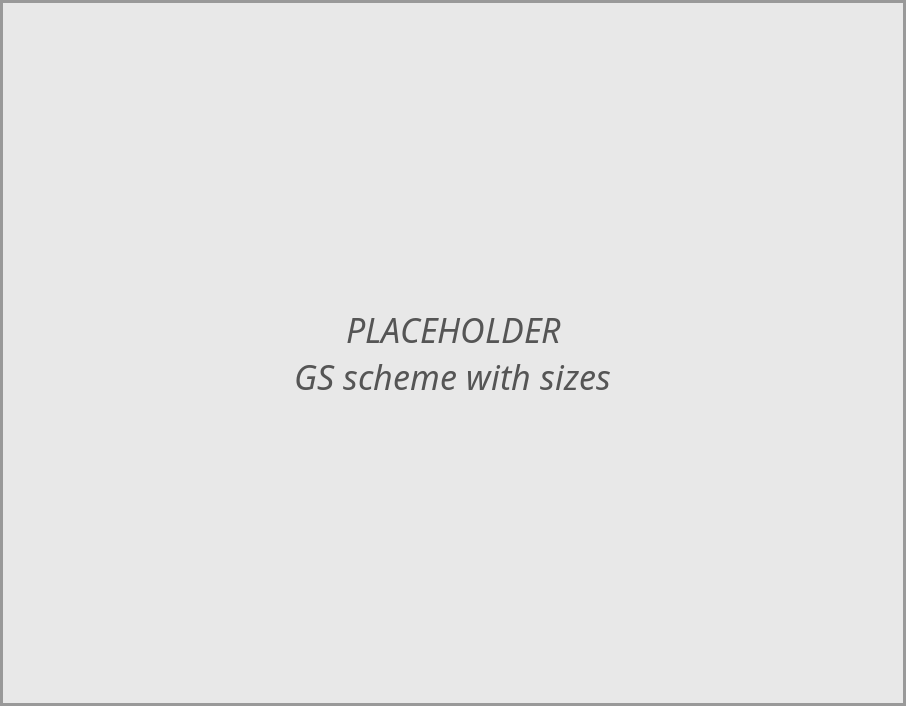
\includegraphics[height=5cm, keepaspectratio]{teams/ground_station/figures/gs_camera_blind_spots.png}
        \label{fig:gs_camera_blind_spots}
    \end{minipage}
    \hfill
    \begin{minipage}[c]{0.49\textwidth}
        \centering
        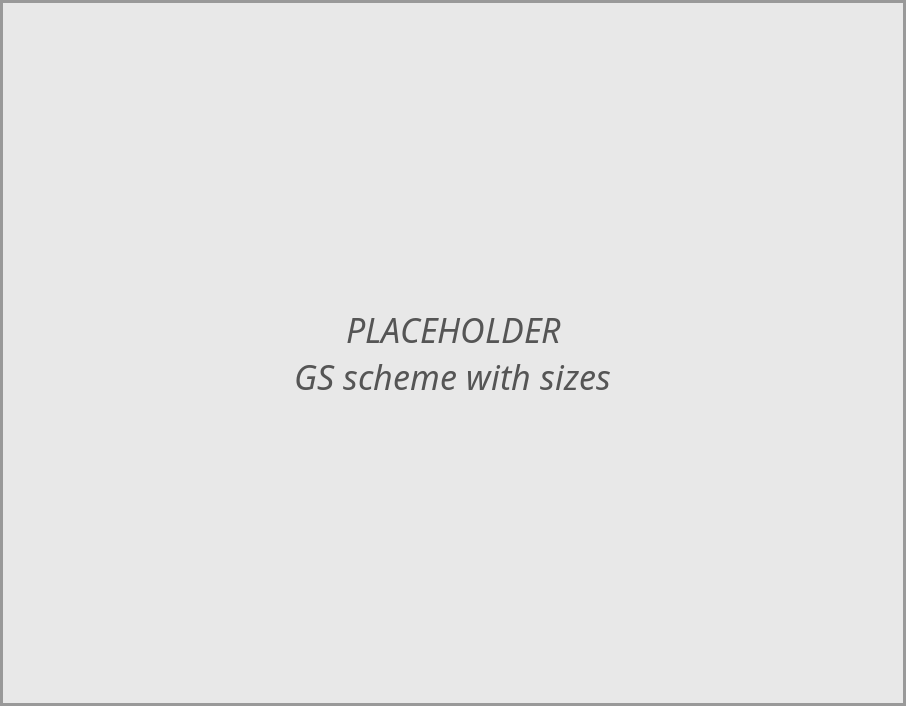
\includegraphics[height=5cm, keepaspectratio]{teams/ground_station/figures/gs_monitor_camera_view.png}
        \label{fig:gs_monitor_camera_view}
    \end{minipage}
    
\end{figure}